\section{Index e login}

Accedendo a \ProjectName{} la prima pagina a cui si è indirizzati è la index page.
Si tratta dell'unica pagina visibile senza aver effettuato l'accesso.

Per effettuare l'accesso è necessario cliccare sul pulsante login in alto a destra.

Come da immagine \ref{loginfig} per potersi autenticare è necessario disporre di un'email e di una password valide.
Non è possibile registrarsi autonomamente nel sistema, dovrà essere l'amministratore ad aggiungere nuovi utenti. Tale procedura sarà illustrata nella sezione \ref{nuovoutente}.

Nel caso in cui i dati inseriti non sono riconosciuti dal sistema verrà restituito un messaggio di errore e l'utente potrà tentare nuovamente la login. Non ci sono limiti sul numero di tentativi possibili.

Se l'autenticazione ha successo si verrà reindirizzati alla pagina Dashboard, illustrata nella sezione \ref{dashboard}
\begin{figure}[h]
	\label{loginfig}
	\centering 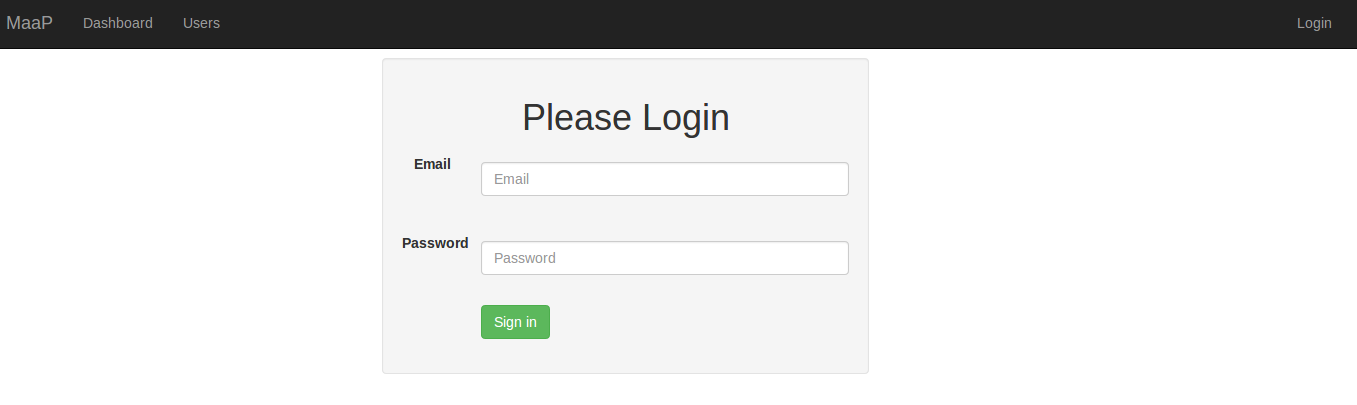
\includegraphics[width=1\textwidth]{login.png}
	\caption{Screen della pagina login.}
\end{figure}

\section{Dashboard}
 \label{dashboard}
 
Si tratta della pagina centrale una volta loggati. Come si vede in figura \ref{dashboardfig} in questa pagina sarà presente un elenco delle collection a cui si ha accesso. Per visualizzare una collection in particolare è sufficiente cliccarci sopra.

\begin{figure}[h]
	\label{dashboardfig}
	\centering 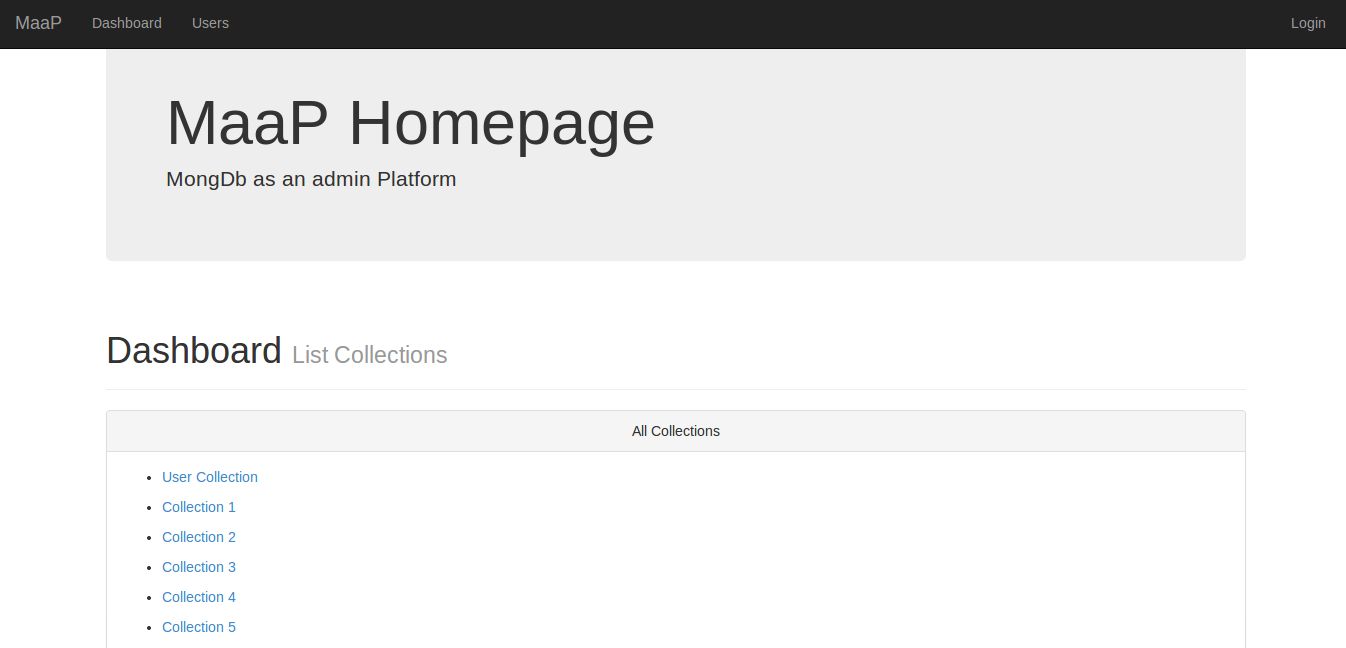
\includegraphics[width=1\textwidth]{dashboard.png}
	\caption{della pagina dashboard. }
\end{figure}

\section{Gestione delle collection}
\subsection{Visualizzare le collection}
\subsection{Gestione dei documenti di una collection}

\section{Gestione utenti}

\begin{figure}[h]
	\centering 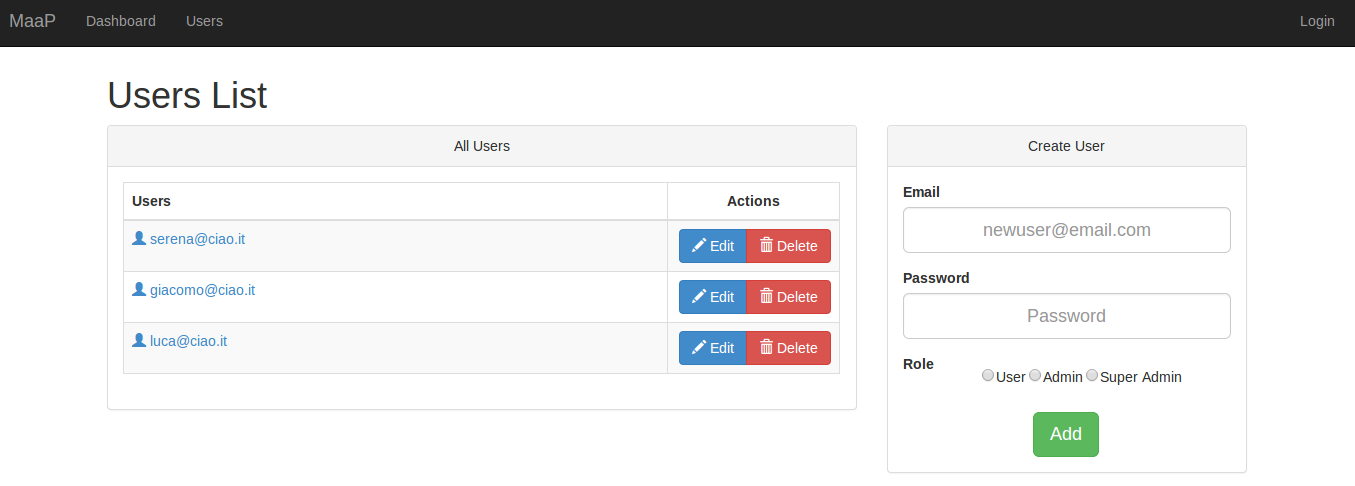
\includegraphics[width=1\textwidth]{userList.png}
	\caption{Screen della pagina userList.}
\end{figure}

\subsection{Visualizzare gli utenti presenti}
\subsection{Registrare nuovi utente}
\label{nuovoutente}
\begin{figure}[h]
	\centering 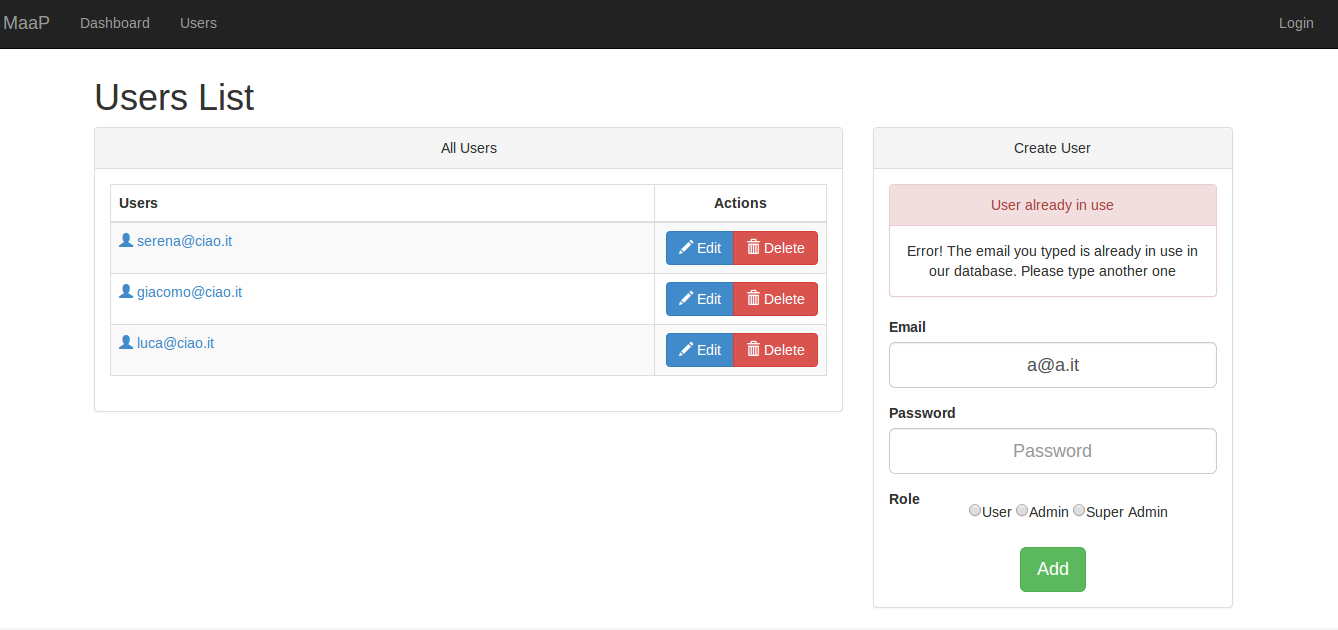
\includegraphics[width=1\textwidth]{userListError.png}
	\caption{Screen della pagina userList con errore. }
\end{figure}

\section{Gestione del profilo personale}





